% Created 2024-02-21 Wed 23:41
% Intended LaTeX compiler: pdflatex
\documentclass[11pt]{article}
\usepackage[utf8]{inputenc}
\usepackage[T1]{fontenc}
\usepackage{graphicx}
\usepackage{longtable}
\usepackage{wrapfig}
\usepackage{rotating}
\usepackage[normalem]{ulem}
\usepackage{amsmath}
\usepackage{amssymb}
\usepackage{capt-of}
\usepackage{hyperref}
\usepackage[T1]{fontenc}
\usepackage{titling}
\usepackage{url}
\usepackage{amsmath,amsthm,amssymb}
\author{Miguel}
\date{\today}
\title{}
\hypersetup{
 pdfauthor={Miguel},
 pdftitle={},
 pdfkeywords={},
 pdfsubject={},
 pdfcreator={Emacs 28.2 (Org mode 9.4.6)}, 
 pdflang={English}}
\begin{document}

\tableofcontents

\documentclass[12pt]{article}
\usepackage{graphicx}
\usepackage{xcolor}
\usepackage{hyperref}
\usepackage{wasysym}
\usepackage{mathrsfs}
\usepackage[calc]{datetime2}
\usepackage{boondox-cal}
\usepackage{bm} \% For bold math symbols
\usepackage{amsmath,amsthm,amssymb,amsbsy}
\usepackage{gensymb}
\usepackage{cancel}
\usepackage{tikz}
\usetikzlibrary{3d,calc}
\usetikzlibrary{arrows}

\DTMsavenow{now}
\DTMsavedate{DueDate}{2024-02-21}

\newcount\daystilldue
\newcount\hourstilldue
\newcount\minutestilldue

\% Calculate the difference in days
\DTMsaveddatediff{DueDate}{now}{\daystilldue}

\% Calculate the difference in hours and minutes
\hourstilldue=\DTMfetchhour{DueDate}
\advance\hourstilldue by -\DTMfetchhour{now}
\minutestilldue=\DTMfetchminute{DueDate}
\advance\minutestilldue by -\DTMfetchminute{now}

\% Adjust for negative values
\ifnum\hourstilldue<0
  \advance\hourstilldue by 24
  \advance\daystilldue by -1
\fi
\ifnum\minutestilldue<0
  \advance\minutestilldue by 60
  \advance\hourstilldue by -1
\fi

\newcommand{\TimeUntilDue}\{
  \ifnum\daystilldue<4
    \textcolor{red}\{
    \number\daystilldue$\backslash$ days - 
    \number\hourstilldue$\backslash$ hours - 
    \number\minutestilldue$\backslash$ min until deadline!!
  \}
\else
    \number\daystilldue$\backslash$ days - 
    \number\hourstilldue$\backslash$ hours - 
    \number\minutestilldue$\backslash$ min until deadline
  \fi
\}



\% Save the original \BibTeX command in case you need it later
\let\originalBibTeX\BibTeX

\% Redefine the \BibTeX command to display the \LaTeX{} logo
\renewcommand{\BibTeX}\{\{\rmfamily B\kern-.03em\{\sffamily ib\}\kern-.15em\TeX\}\}


\newcommand{\delCross}[1]\{
  \left[\hat a\textsubscript{x\left}(\frac\{\(\partial\)\bm{#1}\textsubscript{z}\}\{\(\partial\) y\} - \frac\{\(\partial\)\bm{#1}\textsubscript{y}\}\{\(\partial\) z\}\right) - \hat a\textsubscript{y\left}( \frac\{\(\partial\)\bm{#1}\textsubscript{z}\}\{\(\partial\) x\} - \frac\{\(\partial\)\bm{#1}\textsubscript{x}\}\{\(\partial\) z\}  \right) + \hat a\textsubscript{z\left}( \frac\{\(\partial\)\bm{#1}\textsubscript{y}\}\{\(\partial\) x\} -  \frac\{\(\partial\)\bm{#1}\textsubscript{x}\}\{\(\partial\) y\}\right)\right]
\}
\begin{document}

\newcommand{\Cross}[2]{
\hat a_x(#1_2#2_3 -#1_3#2_2) -\hat a_y(#1_1#2_3-#1_3#2_1) + \hat a_z(#1_1#2_2-#1_2#2_1) 
}
\title{ECE 6310 - Advanced Electromagnetic Fields: Homework Set \#3}
\author{Miguel Gomez}
%\date{\TimeUntilDue}
\maketitle

%\begin{center}
%  $\mathcal{ABCDEFGHIJKLMNOPQRSTUVWXYZ}$\\
%$\mathscr{ABCDEFGHIJKLMNOPQRSTUVWXYZ}$
%\end{center}
\section*{Preliminaries}
In this document, we use standard notation for electromagnetic theory. Key equations and concepts are summarized below:

\subsection*{Vector Notation}
\begin{itemize}
  \item $\bm{\mathcal{E}}$: Electric field intensity
  \item $\bm{\mathcal{H}}$: Magnetic field intensity
  \item $\bm{\mathcal{D}}$: Electric flux density
  \item $\bm{\mathcal{B}}$: Magnetic flux density
  \item $\bm{\mathcal{J}}$: Current density
  \item $\rho_v$: Volume charge density
\end{itemize}

\subsection*{Differential Operators}
\begin{itemize}
  \item $\nabla \cdot\ \ $: Divergence of a vector field
  \item $\nabla \times\ \ $: Curl of a vector field
  \item $\nabla\ \ $: Gradient of a scalar field
  \item $\partial_i\ \ $: Partial derivative with respect to the independent basis element $i$
\end{itemize}

\subsection*{Maxwell's Equations}
In integral form, Maxwell's equations are given by:
\begin{align}
  \oint_{\partial V} \bm{\mathcal{E}} \cdot d\bm{\mathcal{l}} &= - \frac{d}{dt} \int_{V} \bm{\mathcal{B}} \cdot d\bm{\mathcal{S}} & \text{(Faraday's Law of Induction)} \\
  \oint_{\partial V} \bm{\mathcal{H}} \cdot d\bm{\mathcal{l}} &= \int_{V} \bm{\mathcal{J}} \cdot d\bm{\mathcal{S}} + \frac{d}{dt} \int_{V} \bm{\mathcal{D}} \cdot d\bm{\mathcal{S}} & \text{(Ampère's Circuital Law)} \\
  \oiint_{\partial V} \bm{\mathcal{D}} \cdot d\bm{\mathcal{S}} &= \int_{V} \rho_v dV & \text{(Gauss's Law for Electricity)} \\
  \oiint_{\partial V} \bm{\mathcal{B}} \cdot d\bm{\mathcal{S}} &= 0 & \text{(Gauss's Law for Magnetism)}
\end{align}

\subsection*{Other Relevant Equations}
\begin{itemize}
  \item Continuity Equation: $\nabla \cdot \bm{\mathcal{J}} + \partial_t \rho_v = 0$
  \item Relationship between $\bm{\mathcal{E}}$, $\bm{\mathcal{D}}$: $\bm{\mathcal{D}} = \epsilon \bm{\mathcal{E}}$
  \item Relationship between $\bm{\mathcal{H}}$, $\bm{\mathcal{B}}$: $\bm{\mathcal{B}} = \mu \bm{\mathcal{H}}$
\end{itemize}

\subsection*{Boundary Conditions}
Discuss the boundary conditions for $\bm{\mathcal{E}}$, $\bm{\mathcal{H}}$, $\bm{\mathcal{D}}$, and $\bm{\mathcal{B}}$ at interfaces between different media.
\newpage
\section{- 6.19}
Show that for observations made at very large distances $(\beta r \gg 1)$ the electric and magnetic fields of Example 6-3 reduce to the following:
\begin{center}
  \begin{align*}
    E_{\theta} &= j\eta \frac{\beta \bm{I}_e\ell e^{-j\beta r}}{4 \pi r} \sin{(\theta)}\\
    H_{\phi} &\approx \frac{E_{theta}}{\eta}\\
    E_{r} &\approx 0\\
    E_{\phi} &= H_r = H_{\theta} = 0
  \end{align*}
\end{center}
All of the above can be found bf considering a typical hertzian dipole. The example shows that we have an infinitesimal dipole with the length much smaller than a wavelength $\lambda$. Therefore, we can take the expressions as shown with all parts $E$ and $H$ getting a factor of $e^{-j\beta R}$ for the decay, and will have another dependent on the distance from the location of the dipole. We can ignore the factors present in all the values and look to only the factors containin $r^{-1}$.
\begin{align*}
  E_{r} &= A\cdot \left(\frac{1}{r^2}\right)\left(1 + \frac{1}{j\beta r}\right)\\
  &= \left(\frac{1}{r^2} + \frac{1}{j\beta r^3}\right)
\end{align*}
With $r$ being much greater than 1, we can approximate that $E_r \xrightarrow{} 0$ as the distance gets larger.
\begin{align*}
  H_r &= H_{\theta} = 0
\end{align*}
These follow from the reduction of the vector potential equation after converting to spherical. With $A_{phi} = 0$, we do not end up with components in the H direction for these. Then, $H_{phi}$ contains the same factors discussed above and we ignore the ones with higher order $r$'s in the denominator. Leaving us with the same constant multiplied across all terms, but divided by $\eta$, which substituting $E_{theta}$ for that factor gives the expected $H_{phi} \xrightarrow{} \frac{E_{theta}}{\eta}$
\newpage
\section{- 6.20}
For 6.19, show that
\begin{itemize}
\item the time average power density is:
  \begin{align*}
    \mathbf{S} &= \frac{1}{2}\text{Re}{[\mathbf{E}\times\mathbf{H}^*]} = \hat a_r W_{av} = \hat a_r W_{r}\\
    \nabla \times \mathbf{A} &= \frac{1}{r \sin \theta}

  \end{align*}
  \[
\nabla \times \mathbf{A} = \frac{\hat{a}_r}{r \sin \theta}\left[\frac{\partial}{\partial \theta} (A_\phi \sin \theta) - \frac{\partial A_\theta}{\partial \phi}\right] + \frac{\hat{a}_{\theta}}{r}\left[ \frac{\partial r A_r}{\partial \phi} - \frac{\partial A_\phi}{\partial r}\right]
\begin{pmatrix}
 \\
\hat{a}_\phi
\end{pmatrix} \times
\begin{pmatrix}
 \\
 \\
\frac{1}{r} \frac{\partial A_\theta}{\partial r} - \frac{1}{r \sin \theta} \frac{\partial}{\partial \theta} (r A_\phi)
\end{pmatrix}
\]

\item Radiation Intensity
    \begin{align*}
    \mathbf{U} &= r^2S_{av} = \frac{\eta}{8}\left|\frac{\mathbf{I}_o\ell}{\lambda}\right|^2 % more goes here
  \end{align*}
\item Radiated Power
    \begin{align*}
    \mathbf{P}_{rad} &= \int_0^{2\pi}\int_0^{\pi}\mathbf(U)(\theta,\phi)\times \sin{(\theta)}d\thetad\phi = \eta\left(\frac{\pi}{3}\right)\left|\frac{\mathbf{I}_o\ell}{\lambda}\right|^2
  \end{align*}
\item Directivity
  \begin{align*}
    \mathbf{D}_o &=\frac{4\pi\mathbf{U}_{max}(\theta,\phi)}{\mathbf{P}_{rad}} 
  \end{align*}
\item Radiation Resistance
  \begin{align*}
    \mathbf{R}_{rad} &=\frac{2\mathbf{P}_{rad}}{|\mathbf{I}_{0}|^2} = 80\pi^2\left(\frac{\ell}{\lambda}\right)^2 
  \end{align*}
\end{itemize}

\section{- 6.25}
The current distribution on a very thin wire dipole antenna of overall length $\ell$ is given by:
\[
I_e = 
\begin{cases} 
\hat{a} z I_0 \sin [\beta\left(\frac{\ell}{2} - z'\right)] & \text{if } 0 \leq z' \leq \frac{\ell}{2} \\
\hat{a} z I_0 \sin [\beta\left(\frac{\ell}{2} + z'\right)] & \text{if } -\frac{\ell}{2} \leq z' \leq 0
\end{cases}
\]
where I0 is a constant. Representing the distance R of (6-112) by the far-field approximations of (6-112a) through (6-112b), derive the far-zone electric and magnetic fields radiated by the dipole using (6-97a) and the far-field formulations of Section 6.7


\section{- 6.26}
 Show that the radiated far-zone electric and magnetic fields derived in Problem 6.25 reduce for a half-wavelength dipole $(\ell = \frac{\lambda}{2})$ to:
\[
E_{\theta} \approx j \eta \frac{I_0 e^{-j \beta r}}{2\pi r} 
\left[\frac{\cos\left(\frac{\pi}{2} \cos \theta\right)}{
\sin \theta}\right]
\]

\[
H_{\phi} \approx \frac{E_{\theta}}{\eta}
\]

\[
E_r \approx E_{\phi} \approx H_r \approx H_{\theta} \approx 0
\]
*Note: Verify your solutions for the far field $E_{theta}$ for a half-wavelength dipole (6.26) in HFSS; design the antenna to be resonant at $1GHz$.
 
\section{- 6.38}
A coaxial line of inner and outer radii $a$ and $b$, respectively, is mounted on an infinite
conducting ground plane. Assuming that the electric field over the aperture of the coax is:
\[
E_a = -\hat{a}_{\rho} \frac{V}{\varepsilon \ln(\frac{b}{a}) \rho\ '}
\]
\begin{center}
  $\text{where } a \leq \rho\ ' \leq b$
\end{center}
where V is the applied voltage and ε is the permittivity of medium in the coax, find the far-zone spherical electric and magnetic field components radiated by the aperture.
\newpage
\begin{center}
  \begin{tikzpicture}[scale=2,tdplot_main_coords]

    % Define the radii
    \def\innerradius{0.5}
    \def\outerradius{1}
    \def\ellipseangle{0}

    % Draw the annulus as ellipses due to the perspective
    \begin{scope}[rotate=\ellipseangle]
        \shade[inner color=gray!80,outer color=gray!30,opacity=0.75] (0,0) ellipse ({\outerradius} and {0.5*\outerradius});
        \fill[white] (0,0) ellipse ({\innerradius} and {0.3*\innerradius});
    \end{scope}

    % Draw the outer shaded area
    \fill[gray!30,opacity=0.5] (-1.5,-1.5) rectangle (1.75,1.75);

    % Draw the arrows and labels
    \draw[-{Latex[length=3mm]}] (0,0) -- (2.5,0) node[anchor=south east] {$y$};
    \draw[-{Latex[length=3mm]}] (0,0) -- (0,2.5) node[anchor=north west] {$z$};
    \draw[-{Latex[length=3mm]}] (0,0) -- (-1.5,-1.5) node[anchor=north] {$x$};

    % Label the radii and other parameters
    \begin{scope}[rotate=\ellipseangle]
        \draw (0,0) -> node[midway,above] {$a$} (-\innerradius/2,.15);
        \draw (0,0) -> node[midway,above] {$b$} ({-\outerradius/2},.45);
    \end{scope}
    \node[anchor=south] at (0,-.5) {$\varepsilon$};
    \node at (1.3,-1.3) {$\sigma = \infty$};

    % Label the figure
    \node[below] at (current bounding box.south) {Figure P6-38};
\end{tikzpicture}

\end{center}
\section{- 7.3}
An infinitesimal vertical magnetic dipole of length l and constant current Im is placed symmetrically about the origin and it is directed along the z axis, as shown in Figure 6-2 a. Derive expressions valid every- where, near and far field, for the:
\begin{itemize}
\item Electric vector potential components $(F_r , F_{theta} , F_{phi} )$.
\item Electric field components $(E_r , E_{theta} , E_{phi} )$.
\item Magnetic field components $(H_r , H_{theta} , H_{phi} )$.
\item Time-average power density, defined as \\
  \begin{align*}
  \mathbf{S} = \frac{1}{2}\text{Re}{[\mathbf{E}\times\mathbf{H}^*]}
  \end{align*}
\item  Radiation intensity, defined in the far field $U \approx r^2S_{av}$
  \item Power Radiated, defined as \\
  \begin{align*}
  \mathbf{P}_{rad} = \int_0^{2\pi}\int_0^{\pi}U(\theta,\phi)\sin{(\theta)}d\theta d\phi
  \end{align*}
\item Maximum directivity, defined as:
  \begin{align*}
  \mathbf{D}_{0} = \frac{4\pi U(\theta,\phi)}{\mathbf{P}_{rad}}
  \end{align*}
\item Radiation resistance, defined as:
  \begin{align*}
  \mathbf{R}_{r} = \frac{2\mathbf{P}_{rad}}{|I_m|^2}
  \end{align*}
\end{itemize}
\section{- 7.15}
An infinitesimal electric dipole is placed at an angle of $30\degree$ at a height $h$ above a perfectly conducting electric ground plane. Determine the location and orientation of its image. Do this by sketching the image.
\begin{center}
  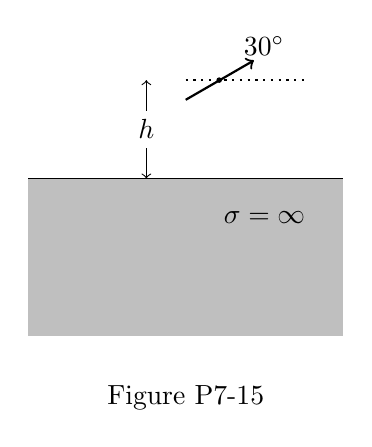
\begin{tikzpicture}

    % Ground
    \fill[gray!50] (-2,-2) rectangle (2,0);
    \draw (-2,0) -- (2,0);

    % Sigma = infinity
    \node at (1,-0.5) {$\sigma = \infty$};

    % Antenna
    \draw[thick, dotted] (0,1.25) -- (1.5,1.25);
    \draw[->,thick] (0,1) -- +(30:1) node[midway, above right, xshift=.5em, yshift=.5em] {30$^\circ$};
    \fill (.425,1.25) circle (1pt);
    % Height
    \draw[<->] (-0.5,0) -- node[midway, fill=white] {$h$} (-0.5,1.25);

    % Label
    \node[below] at (0,-2.5) {Figure P7-15};

\end{tikzpicture}

\end{center}
\section{- 7.37}
For the aperture shown in Figure 6-4c and
assuming it is mounted on an infinite PEC
ground plane:
\begin{itemize}
\item [a)] Form the most practical, exact or approximate (when necessary to solve the problem), equivalent currents $\mathbf{J}_s$ and $\mathbf{M}_s$.
\item [b)] Find the far-zone electric and magnetic fields. The electric field distribution at the aperture is given by ($Eo$ is a constant):\\
  \begin{align*}
    \mathbf{E}_a &= \hat a_yE_0\\
    -\frac{a}{2} \le x\ ' \le \frac{a}{2}\ \ \ &;\ \ \ -\frac{b}{2} \le y\ ' \le \frac{b}{2}
  \end{align*}
\end{itemize}
\bibliographystyle{plain}
\bibliography{references/references}

\end{document}

\%\%\% Local Variables:
\%\%\% mode: \LaTeX{}
\%\%\% \TeX{}-master: t
\%\%\% End:
\end{document}